\documentclass{article}
\usepackage{pgfplots}
\pgfplotsset{compat=1.18}

\begin{document}

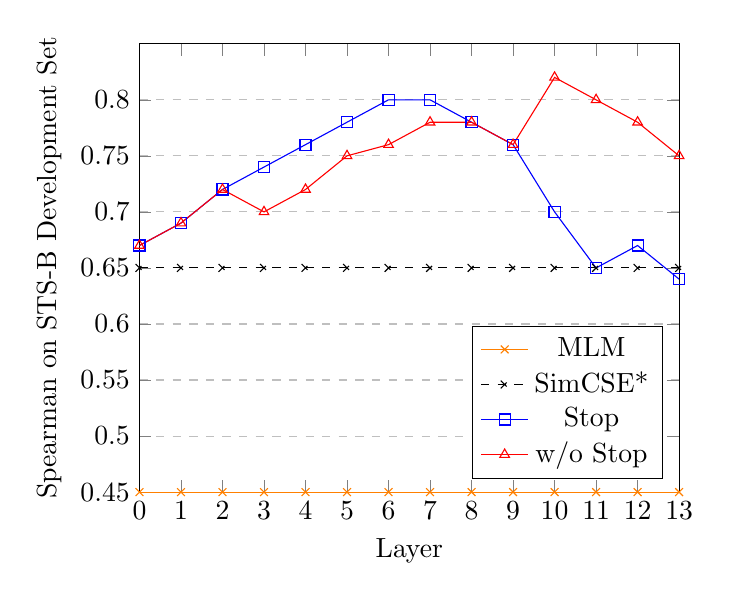
\begin{tikzpicture}
    \begin{axis}[
        xlabel={Layer},
        ylabel={Spearman on STS-B Development Set},
        xmin=0, xmax=13,
        ymin=0.45, ymax=0.85,
        xtick={0,1,...,13},
        ytick={0.45, 0.5, ..., 0.85},
        legend pos=south east,
        ymajorgrids=true,
        grid style=dashed,
    ]
    
    % MLM
    \addplot[
        color=orange,
        mark=x,
        ]
        coordinates {
            (0,0.45)(1,0.45)(2,0.45)(3,0.45)(4,0.45)(5,0.45)(6,0.45)(7,0.45)(8,0.45)(9,0.45)(10,0.45)(11,0.45)(12,0.45)(13,0.45)
        };
        \addlegendentry{MLM}
        
    % SimCSE*
    \addplot[
        color=black,
        dashed,
        mark=x,
        ]
        coordinates {
            (0,0.65)(1,0.65)(2,0.65)(3,0.65)(4,0.65)(5,0.65)(6,0.65)(7,0.65)(8,0.65)(9,0.65)(10,0.65)(11,0.65)(12,0.65)(13,0.65)
        };
        \addlegendentry{SimCSE*}
        
    % Stop
    \addplot[
        color=blue,
        mark=square,
        ]
        coordinates {
            (0,0.67)(1,0.69)(2,0.72)(3,0.74)(4,0.76)(5,0.78)(6,0.80)(7,0.80)(8,0.78)(9,0.76)(10,0.70)(11,0.65)(12,0.67)(13,0.64)
        };
        \addlegendentry{Stop}
        
    % w/o Stop
    \addplot[
        color=red,
        mark=triangle,
        ]
        coordinates {
            (0,0.67)(1,0.69)(2,0.72)(3,0.70)(4,0.72)(5,0.75)(6,0.76)(7,0.78)(8,0.78)(9,0.76)(10,0.82)(11,0.80)(12,0.78)(13,0.75)
        };
        \addlegendentry{w/o Stop}
        
    \end{axis}
\end{tikzpicture}

\end{document}